%!TEX root = ../../thesis.tex
\section{Structure}

The backend implementation is based on a micro framework that has been developed on top of Express and bases itself loosely on the MVC pattern. It is a stateless framework and deals with HTTP connections for all requests that are not related to the synchronization module. The synchronization module uses WebSockets instead of HTTP.

\begin{figure}[htb]
  \centerline{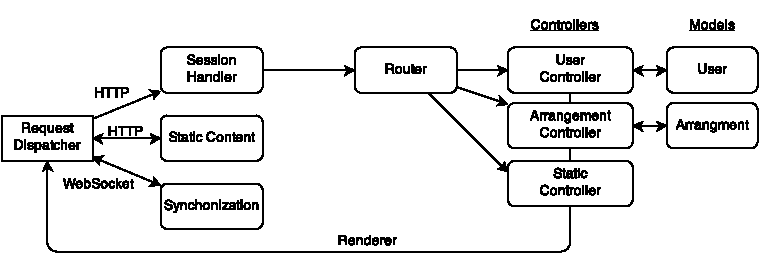
\includegraphics[width=\linewidth]{images/BackendDiagram.pdf}}
  \caption[The backend structure]{The backend structure}
  \label{fig:backend-structure}
\end{figure}

All requests are handled by the `Request Dispatcher' which, dependent on the URL and the type of the request (HTTP vs WebSocket), decides to which module the request will be forwarded. The simplest module is the `Static Content' module, because it simply loads all static files like the frontend JavaScript and the CSS from disk and delivers it to the client. It also takes care of delivering all uploaded audio files.

The synchronization module is initialized by WebSocket connections and it handles all sync-relevant operations which are explained in more detail in \refchapter{impl-sync-algorithm}.

Requests that are not handled by the two already mentioned modules are passed on to the `Session Handler' and the `Router'. The `Session Handler' ensures that all requests that reach the `Router' have a session attached to it so that they can be associated with a user. The `Router' basically consists of a `URL to Controller' lookup table and passes the request on to the `Controller' that is associated to the address of the current request. There are three main controllers. The `StaticSite' controller takes care of rendering the website's views into HTML. The `User' controller deals with sign-ups and rendering the user pages. The `Arrangement' controller creates and renders project files. All controllers have models associated that take care of the basic CRUD\footnote{Create Retrieve Update Delete} operations with the database.

The architecture of the framework has been developed in a modular way so that it can be reused for other websites as well. In order to implement a normal website that does not need the synchronization module, the module only needs to be removed and the framework can be used without it.